\documentclass[journal,12pt,twocolumn]{IEEEtran}
%
\usepackage{setspace}
\usepackage{gensymb}
\singlespacing
\usepackage[cmex10]{amsmath}
\usepackage{siunitx}
\usepackage{amsthm}

\usepackage{mathrsfs}

\usepackage{txfonts}
\usepackage{stfloats}

\usepackage{steinmetz}
\usepackage{cite}
\usepackage{cases}
\usepackage{subfig}
\usepackage{longtable}
\usepackage{multirow}
\usepackage{enumitem}
\usepackage{mathtools}
\usepackage{tikz}
\usepackage{circuitikz}
\usepackage{verbatim}
\usepackage{tfrupee}
\usepackage[breaklinks=true]{hyperref}
\usepackage{tkz-euclide} % loads  TikZ and tkz-base
\usetikzlibrary{calc,math}
\usetikzlibrary{fadings}
\usepackage{listings}
    \usepackage{color}                                            %%
    \usepackage{array}                                            %%
    \usepackage{longtable}                                        %%
    \usepackage{calc}                                             %%
    \usepackage{multirow}                                         %%
    \usepackage{hhline}                                           %%
    \usepackage{ifthen}                                           %%
  %optionally (for landscape tables embedded in another document): %%
    \usepackage{lscape}     
\usepackage{multicol}
\usepackage{chngcntr}
\DeclareMathOperator*{\Res}{Res}

\renewcommand\thesection{\arabic{section}}
\renewcommand\thesubsection{\thesection.\arabic{subsection}}
\renewcommand\thesubsubsection{\thesubsection.\arabic{subsection}}

\renewcommand\thesectiondis{\arabic{section}}
\renewcommand\thesubsectiondis{\thesectiondis.\arabic{subsubsection}}
\renewcommand\thesubsubsectiondis{\thesubsectiondis.\arabic{subsubsection}}

\hyphenation{op-tical net-works semi-conduc-tor}
\def\inputGnumericTable{}                                 %%

\lstset{
%language=C,
frame=single, 
breaklines=true,
columns=fullflexible
}
\begin{document}
%


\newtheorem{theorem}{Theorem}[section]
\newtheorem{problem}{Problem}
\newtheorem{proposition}{Proposition}[section]
\newtheorem{lemma}{Lemma}[section]
\newtheorem{corollary}[theorem]{Corollary}
\newtheorem{example}{Example}[section]
\newtheorem{definition}[problem]{Definition}

\newcommand{\BEQA}{\begin{eqnarray}}
\newcommand{\EEQA}{\end{eqnarray}}
\newcommand{\define}{\stackrel{\triangle}{=}}
\bibliographystyle{IEEEtran}
\providecommand{\mbf}{\mathbf}
\providecommand{\pr}[1]{\ensuremath{\Pr\left(#1\right)}}
\providecommand{\qfunc}[1]{\ensuremath{Q\left(#1\right)}}
\providecommand{\sbrak}[1]{\ensuremath{{}\left[#1\right]}}
\providecommand{\lsbrak}[1]{\ensuremath{{}\left[#1\right.}}
\providecommand{\rsbrak}[1]{\ensuremath{{}\left.#1\right]}}
\providecommand{\brak}[1]{\ensuremath{\left(#1\right)}}
\providecommand{\lbrak}[1]{\ensuremath{\left(#1\right.}}
\providecommand{\rbrak}[1]{\ensuremath{\left.#1\right)}}
\providecommand{\cbrak}[1]{\ensuremath{\left\{#1\right\}}}
\providecommand{\lcbrak}[1]{\ensuremath{\left\{#1\right.}}
\providecommand{\rcbrak}[1]{\ensuremath{\left.#1\right\}}}
\theoremstyle{remark}
\newtheorem{rem}{Remark}
\newcommand{\sgn}{\mathop{\mathrm{sgn}}}
\providecommand{\abs}[1]{\$left\vert#1\$right\vert}
\providecommand{\res}[1]{\Res\displaylimits_{#1}} 
\providecommand{\norm}[1]{\$left\lVert#1\$right\rVert}
%\providecommand{\norm}[1]{\lVert#1\rVert}
\providecommand{\mtx}[1]{\mathbf{#1}}
\providecommand{\mean}[1]{E\$left[ #1 \$right]}
\providecommand{\fourier}{\overset{\mathcal{F}}{ \rightleftharpoons}}
%\providecommand{\hilbert}{\overset{\mathcal{H}}{ \rightleftharpoons}}
\providecommand{\system}{\overset{\mathcal{H}}{ \longleftrightarrow}}
	%\newcommand{\solution}[2]{\textbf{Solution:}{#1}}
\newcommand{\solution}{\noindent \textbf{Solution: }}
\newcommand{\cosec}{\,\text{cosec}\,}
\providecommand{\dec}[2]{\ensuremath{\overset{#1}{\underset{#2}{\gtrless}}}}
\newcommand{\myvec}[1]{\ensuremath{\begin{pmatrix}#1\end{pmatrix}}}
\newcommand{\mydet}[1]{\ensuremath{\begin{vmatrix}#1\end{vmatrix}}}
\numberwithin{equation}{subsection}
\makeatletter
\@addtoreset{figure}{problem}
\makeatother
\let\StandardTheFigure\thefigure
\let\vec\mathbf
\renewcommand{\thefigure}{\theproblem}
\def\putbox#1#2#3{\makebox[0in][l]{\makebox[#1][l]{}\raisebox{\baselineskip}[0in][0in]{\raisebox{#2}[0in][0in]{#3}}}}
     \def\rightbox#1{\makebox[0in][r]{#1}}
     \def\centbox#1{\makebox[0in]{#1}}
     \def\topbox#1{\raisebox{-\baselineskip}[0in][0in]{#1}}
     \def\midbox#1{\raisebox{-0.5\baselineskip}[0in][0in]{#1}}
\vspace{3cm}
\title{ASSIGNMENT-3}

\maketitle
\newpage
\bigskip
\renewcommand{\thefigure}{\theenumi}
\renewcommand{\thetable}{\theenumi}
% 
Find the python code from below link
% 
\begin{lstlisting}
https://raw.githubusercontent.com/TGURUBALAJI/INTERNSHIP-IITH/main/Assignment%20-3/code.py
\end{lstlisting}
% 
Find the Latex code from below link
% 
\begin{lstlisting}
https://raw.githubusercontent.com/TGURUBALAJI/INTERNSHIP-IITH/main/Assignment%20-3/code.py
\end{lstlisting}

\section{QUESTION NO-3}
 \noindent \myvec{-3 , -2} and \myvec{-6 , 7}, the axes being inclined at \ang{60}.\\  
 
 \
 \\{Solution}
 :
 \vec{A}=\myvec{-3 \\ -2} , \vec{B} =\myvec{-6 \\ 7}
 
 axes being incline at \ang{60} formula for linear transformation from angular coordinates 
 $X = PX_{n}$

\begin{align}
	where\ X= coordinates\ in \ linear \ coordinates\\
	X_{n}=Angular\ coordinates
\end{align}

\begin{figure}[!h]
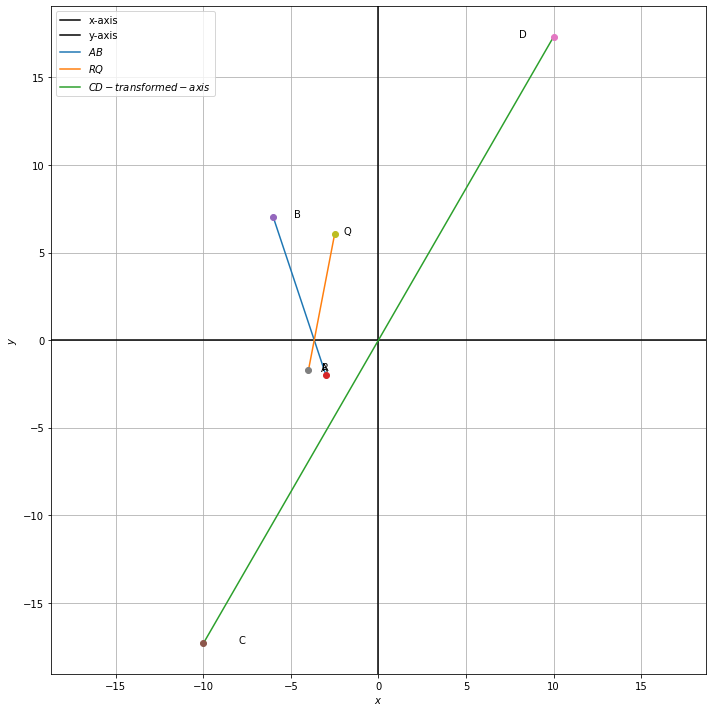
\includegraphics[width=\columnwidth]{Dis btw two points.png}
\caption{$transformed \ lines$}
\label{fig:straight lines}	
\end{figure}
\begin{align}
\vec{P} &=\myvec{1 & \cos{(\theta)}\\ 0 & \sin{(\theta)}}\\
\vec{A} &=\myvec{1 & \cos{(\ang{60} )}\\ 0 & \sin{(\ang{60} )}} \myvec{-3 \\ -2}\\
\vec{A} &=\myvec{-3 -2\cos{(\ang{60} )}\\  -2\sin{(\ang{60} )}} \\
\vec{B} &=\myvec{1 & \cos{(\ang{60} )}\\ 0 & \sin{(\ang{60} )}} \myvec{-6 \\ 7}\\
\vec{B} &=\myvec{-6 +7\cos{(\ang{60} )}\\  7\sin{(\ang{60} )}} 
\end{align}
distance between two points is given by
\begin{align}
$||\vec{A}-\vec{B}||$ &= \sqrt{(\vec{A}-\vec{B})^{T}(\vec{A}-vec{B})}\\

\vec{A}-\vec{B} &=\myvec{-3 -2\cos{(\ang{60} )}\\  -2\sin{(\ang{60} )}} - \myvec{-6 +7\cos{(\ang{60} )}\\  7\sin{(\ang{60} )}}\\

\vec{A}-\vec{B} &=\myvec{3 -9\cos{(\ang{60} )}\\  -9\sin{(\ang{60} )}} 

$||\vec{A}-\vec{B}||$ &=\sqrt{\myvec{3-9\cos{\ang{60} & -9\sin{\ang{60}}}} \ \myvec{3 -9\cos{(\ang{60} )}\\  -9\sin{(\ang{60} )}} }\\

$||\vec{A}-\vec{B}||$&=\sqrt{(3-9\cos{\ang{60}})^{2}+(-9\sin{\ang{60}})^{2})}\\
\end{align}


\begin{align}

$||\vec{A}-\vec{B}||$ &=\sqrt{9+ 81\cos^{2}{\ang{60}}-54\cos{60}+81\sin^{2}{\ang{60}})}\\

$||\vec{A}-\vec{B}||$ &=\sqrt{9+ 81-54\cos{60}}\\	

$||\vec{A}-\vec{B}||$ &=\sqrt{90 - 27}\\	

$||\vec{A}-\vec{B}||$ &=\sqrt{63}\\	

$||\vec{A}-\vec{B}||$ &=7.9372	

Distance between two points is 7.9372 .
\end{align}
\end{document}
